\section{Results}
In this section we present a comparison of the CVP projector with the TT projector and with a ray casting projector based on Siddon's algorithm of comparable accuracy. When studying the view-dependent accuracy of the projectors, we compared the CVP projector with the \texttt{SiddonK} algorithm, see Section \ref{sec:perpixel}, where $K$ was chosen as a power of $2$ ranging from $1$ to $512$. We noticed that a projector showing similar accuracy to the CVP projector is the \texttt{Siddon8} projector, where we cast $64$ rays towards each pixel. Therefore, in what follows we will compare the CVP, its relaxed version, the TT projector and the \texttt{Siddon8} projector in terms of speed and accuracy. For simplicity, we present only the results for CVP with elevation correction. Elevation correction can also be turned off to increase speed at the cost of the reduced accuracy.

\subsection{Comparison of the speed}
To compare the speed of the projectors, we found two examples from the literature where the authors report the TT projector speed of their algorithms. Based on these problems, we created sets of projection geometries and two benchmarks to compare the speeds of our projectors. For comparison, we also provide the times reported in the papers, but it is clear that they were created on different hardware and with different settings for the specific data projected.

We derived the first benchmark problem from the setup in \cite{Long2010}. The arrangement is determined by a circular CT trajectory with a flat detector, where the distance from the source to the detector is 949mm and the distance from the source to the isocenter is 541mm, and where 720 views are equally spaced around the circular trajectory. Detector matrix of the device consists of $512 \times 512$ detector cells of the dimensions $\SI{1.0}{\milli \meter} \times \SI{1.0}{\milli \meter}$. Volume dimensions are $512 \times 512 \times 128$ with the voxel size $\SI{0.5}{\milli\meter} \times \SI{0.5}{\milli \meter} \times \SI{0.5}{\milli \meter}$. Thus, the vector $\vec{x}$ for the reconstruction problem \eqref{eq:fundament} has $512 \cdot 512 \cdot 128 = 33.5M$ elements and the vector $\vec{b}$ has $512 \cdot 512 \cdot 720 = 188.7M$ elements. Long et. al. \cite{Long2010} reported the best time of the TT projector as \SI{91}{\second}, the best time of the backprojector as \SI{93}{\second}. It was not explicitly stated that 720 views were used for this comparison, but we assume so from the text of the previous paragraph in the linked article. Our projector speed comparison is summarised in the Table \ref{speed:long}.

% \begin{table}[]
% \caption{Comparison of the speed of the projectors and backprojectors with the same setup as in \cite{Long2010} p.~1846, Table II, where for TT projector authors reported projection time \SI{91}{\sec} and backprojection time \SI{93}{\sec}. }
% \centering
% \begin{tabular}{@{}lSSSS@{}}
% \toprule
%                     & \multicolumn{2}{l}{AMD Radeon VII} & \multicolumn{2}{l}{NVIDIA 2080 Ti} \\ \midrule
%                     & \multicolumn{1}{c}{P}      & \multicolumn{1}{c}{BP}      & \multicolumn{1}{c}{P}         & \multicolumn{1}{c}{BP}        \\
% bar\_norel\_elv     & \SI{37.6}{\second}          & \SI{19.7}{\second}             &      \SI{166.8}{\second}            &        \SI{84.8}{\second}            \\
% bar\_norel\_noelv   & \SI{29.8}{\second}           & \SI{13.8}{\second}             &     \SI{93.0}{\second}             &       \SI{49.9}{\second}              \\
% bar\_rel\_elv       & \SI{12.3}{\second}          & \SI{5.2}{\second}              &    \SI{12.8}{\second}              &       \SI{4.5}{\second}              \\
% bar\_rel\_noelv     & \SI{12.3}{\second}          & \SI{4.4}{\second}              & \SI{11.1}{\second}            & \SI{4.6}{\second}                \\
% nobar\_norel\_elv   & \SI{39.3}{\second}          & \SI{19.7}{\second}             &     \SI{154.1}{\second}             &          \SI{86.6}{\second}           \\
% nobar\_norel\_noelv & \SI{36.9}{\second}          & \SI{13.8}{\second}             &    \SI{75.2}{\second}              &       \SI{50.2}{\second}              \\
% nobar\_rel\_elv     & \SI{30.9}{\second}          &    \SI{5.2}{\second}               &    \SI{18.3}{\second}              &    \SI{4.5}{\second}                 \\
% nobar\_rel\_noelv   & \SI{29.3}{\second}               &    \SI{4.4}{\second}               &     \SI{17.1}{\second}             &    \SI{4.5}{\second}                 \\
% TT                  &  \SI{101.1}{\second}          &  \SI{18.8}{\second}                 &   \SI{312.0}{\second}                &\SI{101.6}{\second}   \\    
% Siddon8                  &      \SI{117.8}{\second}     &  \SI{244.2}{\second}                &    \SI{310.0}{\second}              & \SI{101.1}{\second} \\    \bottomrule
% \end{tabular}
% \end{table}



\begin{table}[]
\caption{Comparison of the speed of the projectors and backprojectors with settings as described in \cite{Long2010} p.~1846, Table II, where for TT projector authors reported projection time \SI{91}{\sec} and backprojection time \SI{93}{\sec}. }
\label{speed:long}
\centering
\begin{tabular}{@{}lSSSS@{}}
\toprule
                    & \multicolumn{2}{l}{AMD Radeon VII} & \multicolumn{2}{l}{NVIDIA 2080 Ti} \\ \midrule
                    & \multicolumn{1}{c}{P}      & \multicolumn{1}{c}{BP}      & \multicolumn{1}{c}{P}         & \multicolumn{1}{c}{BP}        \\
%nobar\_norel\_elv
CVP   & \SI{39.3}{\second}          & \SI{19.7}{\second}             &     \SI{154.1}{\second}             &          \SI{86.6}{\second}           \\
%bar\_rel\_elv
\rowcolor{yellow!50}
CVP relaxed       & \SI{12.3}{\second}          & \SI{5.2}{\second}              &    \SI{12.8}{\second}              &       \SI{4.5}{\second}   \\
TT                  &  \SI{101.1}{\second}          &  \SI{18.8}{\second}                 &   \SI{312.0}{\second}                &\SI{101.6}{\second}   \\    
\texttt{Siddon8}                   &      \SI{117.8}{\second}     &  \SI{244.2}{\second}                &    \SI{310.0}{\second}              & \SI{101.1}{\second} \\   \bottomrule
\end{tabular}
\end{table}

We derived the second benchmark problem from the setup in \cite{Pfeiffer2021}. The arrangement is determined by a circular CT trajectory with a flat detector, where the distance from the source to the detector is \SI{1000}{\milli \meter} and the distance from the source to the isocenter is \SI{750}{\milli \meter}, and where 100 views are equally spaced around the \SI{198}{\degree} part of the circular trajectory. Detector matrix of the device consists of $1280 \times 960$ detector cells of the dimensions $\SI{0.25}{\milli \meter} \times \SI{0.25}{\milli \meter}$. Volume dimensions are $256 \times 256 \times 256$ with the voxel size $\SI{0.5}{\milli\meter} \times \SI{0.5}{\milli \meter} \times \SI{0.5}{\milli \meter}$. Thus, the vector $\vec{x}$ for the reconstruction problem \eqref{eq:fundament} has $256 \cdot 256 \cdot 256 = 16.8M$ elements and the vector $\vec{b}$ has $1280 \cdot 960 \cdot 100 = 122.9M$ elements. Pfeiffer et. al. \cite{Pfeiffer2021} reported the time of the TT projector as \SI{46.3}{\second}, backprojector time was not disclosed. Our projector speed comparison is summarised in the Table \ref{speed:pfeiffertest}.

%Projecting ones
% \begin{table}[]
% \caption{Comparison of the speed of the projectors and backprojectors with the same setup as in \cite{Pfeiffer2021}, Table 1, where for TT projector authors reported projection time \SI{46.3}{\sec}, backprojection time was not disclosed. }
% \centering
% \begin{tabular}{@{}lSSSS@{}}
% \toprule
%                     & \multicolumn{2}{l}{AMD Radeon VII} & \multicolumn{2}{l}{NVIDIA 2080 Ti} \\ \midrule
%                     & \multicolumn{1}{c}{P}      & \multicolumn{1}{c}{BP}      & \multicolumn{1}{c}{P}         & \multicolumn{1}{c}{BP}        \\
% bar\_norel\_elv     & \SI{27.2}{\second}          & \SI{14.0}{\second}              &      \SI{112.1}{\second}            &        \SI{69.6}{\second}             \\
% bar\_norel\_noelv   & \SI{20.2}{\second}           & \SI{9.1}{\second}             &    \SI{66.5}{\second}             &       \SI{38.7}{\second}               \\
% bar\_rel\_elv       &\SI{7.5}{\second}           & \SI{4.1}{\second}             &    \SI{9.3}{\second}            &       \SI{3.4}{\second}              \\
% bar\_rel\_noelv     & \SI{6.8}{\second}         & \SI{3.1}{\second}               & \SI{8.2}{\second}          & \SI{2.6}{\second}                \\
% nobar\_norel\_elv   &\SI{0}{\second}           & \SI{0}{\second}            &     \SI{90.7}{\second}             &          \SI{67.8}{\second}          \\
% nobar\_norel\_noelv & \SI{0}{\second}          & \SI{0}{\second}             &   \SI{55.4}{\second}            &       \SI{37.8}{\second}             \\
% nobar\_rel\_elv     &\SI{0}{\second}          &    \SI{0}{\second}               &   \SI{9.4}{\second}             &    \SI{3.3}{\second}                 \\
% nobar\_rel\_noelv   &\SI{0}{\second}               &    \SI{0}{\second}               &    \SI{9.0}{\second}           &   \SI{2.4}{\second}                 \\
% TT                  &  \SI{29.0}{\second}        &  \SI{11.3}{\second}               &     \SI{120.6}{\second}             & \SI{68.0}{\second} \\    
% Siddon8                  &      \SI{284.6}{\second}     &  \SI{677.0}{\second}           &                  &  \\    \bottomrule
% \end{tabular}
% \end{table}

% \begin{table}[]
% \caption{Comparison of the speed of the projectors and backprojectors with the same setup as in \cite{Pfeiffer2021}, Table 1, where for TT projector authors reported projection time \SI{46.3}{\sec}, backprojection time was not disclosed. }
% \centering
% \begin{tabular}{@{}lSSSS@{}}
% \toprule
%                     & \multicolumn{2}{l}{AMD Radeon VII} & \multicolumn{2}{l}{NVIDIA 2080 Ti} \\ \midrule
%                     & \multicolumn{1}{c}{P}      & \multicolumn{1}{c}{BP}      & \multicolumn{1}{c}{P}         & \multicolumn{1}{c}{BP}        \\
% bar\_norel\_elv     & \SI{27.2}{\second}          & \SI{13.9}{\second}              &      \SI{106.7}{\second}            &        \SI{66.3}{\second}             \\
% bar\_norel\_noelv   & \SI{20.2}{\second}           & \SI{9.0}{\second}             &    \SI{64.8}{\second}             &       \SI{37.7}{\second}               \\
% bar\_rel\_elv       &\SI{7.5}{\second}           & \SI{4.1}{\second}             &    \SI{9.3}{\second}            &       \SI{3.4}{\second}              \\
% bar\_rel\_noelv     & \SI{6.7}{\second}         & \SI{3.1}{\second}               & \SI{7.2}{\second}          & \SI{2.5}{\second}                \\
% nobar\_norel\_elv   &\SI{22.5}{\second}           & \SI{14.1}{\second}            &     \SI{88.9}{\second}             &          \SI{66.8}{\second}          \\
% nobar\_norel\_noelv & \SI{20.5}{\second}          & \SI{9.3}{\second}             &   \SI{88.9}{\second}            &       \SI{66.8}{\second}             \\
% nobar\_rel\_elv     &\SI{17.7}{\second}          &    \SI{4.1}{\second}               &   \SI{9.3}{\second}             &    \SI{3.2}{\second}                 \\
% nobar\_rel\_noelv   &\SI{17.4}{\second}               &    \SI{3.1}{\second}               &    \SI{9.3}{\second}           &   \SI{2.6}{\second}                 \\
% TT                  &  \SI{27.6}{\second}        &  \SI{11.5}{\second}               &     \SI{120.6}{\second}             & \SI{68.0}{\second} \\    
% Siddon8                  &      \SI{282.2}{\second}     &  \SI{684.5}{\second}           &    \SI{942.1}{\second}              &  \SI{1911.6}{\second}\\    \bottomrule
% \end{tabular}
% \end{table}

\begin{table}[]
\caption{Comparison of the speed of the projectors and backprojectors with settings as described in \cite{Pfeiffer2021}, Table 1, where for TT projector authors reported projection time \SI{46.3}{\sec}, backprojection time was not disclosed. }
\label{speed:pfeiffertest}
\centering
\begin{tabular}{@{}lSSSS@{}}
\toprule
                    & \multicolumn{2}{l}{AMD Radeon VII} & \multicolumn{2}{l}{NVIDIA 2080 Ti} \\ \midrule
                    & \multicolumn{1}{c}{P}      & \multicolumn{1}{c}{BP}      & \multicolumn{1}{c}{P}         & \multicolumn{1}{c}{BP}        \\
CVP   &\SI{22.5}{\second}           & \SI{14.1}{\second}            &     \SI{88.9}{\second}             &          \SI{66.8}{\second}          \\
%bar\_rel\_elv
\rowcolor{yellow!50}
CVP relaxed &\SI{7.5}{\second}           & \SI{4.1}{\second}             &    \SI{9.3}{\second}            &       \SI{3.4}{\second}              \\
TT                 &  \SI{27.6}{\second}        &  \SI{11.5}{\second}               &     \SI{120.6}{\second}             & \SI{68.0}{\second} \\   
\texttt{Siddon8}                   &      \SI{282.2}{\second}     &  \SI{684.5}{\second}           &    \SI{942.1}{\second}              &  \SI{1911.6}{\second}\\    \bottomrule
\end{tabular}
\end{table}

To test the speed of the projectors and backprojectors, random projection data was generated from a uniform distribution $[0,1]$. These were then used as input for 40 iterations of the reconstruction algorithm (CGLS). The average projector and backprojector times within the reconstruction were measured. The reported times thus do not include times of I/O operations associated with loading data into the GPU card memory and reading the GPU card memory into the final result. These are just one-time operations within the reconstruction that take on the order of seconds depending on the storage device used.

\subsection{Comparison of the accuracy}
To compare the accuracy of the projectors, we observe the projection of a single voxel onto the detector as a function of rotation angle over a circular trajectory with 360 views. To obtain ground truth data, we used the \texttt{Siddon512} projector, which uses 262,144 rays casted towards each pixel.

Let $\mathbf{P}^{S} \in \mathbb{R}^{M \times N}$ and $\mathbf{P}^{PRJ} \in \mathbb{R}^{M \times N}$ be the matrices representing the data from a given view for \texttt{Siddon512} and a projector PRJ, respectively. Frobenius norm of the matrix $\mathbf{P}$ is
\begin{equation}
    \|\mathbf{P}\| = \sqrt{\sum_{m=0}^{M-1} \sum_{n=0}^{N-1} \mathbf{P}^2_{m,n}}.
\end{equation}
%this norm is often called the L2 norm since the projection data are treated as vectors.
We introduce the relative projector error of PRJ for a given view as 
\begin{equation}
    e_{PRJ} = \frac{\|\mathbf{P}^{PRJ}-\mathbf{P}^{S}\|}{\|\mathbf{P}^{S}\|},
\end{equation}
the reported error in percent is given by $100\cdot e_{PRJ}$.

We studied the relative error of the projector for two different configurations. The first arrangement uses a fine detector grid in a CBCT setup, where the distance from the source to the isocenter is $\SI{749}{\milli \meter}$ and the distance from source to the detector is $\SI{1198}{\milli \meter}$. Detector matrix of the device consists of $616 \times 480$ detector cells of the dimensions $\SI{0.154}{\milli \meter} \times \SI{0.154}{\milli \meter}$. In Figure \ref{fig:projectorerror} top, there is an error profile of the voxel $\SI{1}{\milli \meter} \times \SI{1}{\milli \meter} \times \SI{5}{\milli \meter}$ positioned in the center of rotation. In Figure \ref{fig:projectorerror} in the middle, the voxel $\SI{1}{\milli \meter} \times \SI{1}{\milli \meter} \times \SI{1}{\milli \meter}$ is shifted in the direction of the corner, so that it is still visible on the detector from all views, its center has the coordinates $\SI{20}{\milli \meter} \times \SI{20}{\milli \meter} \times \SI{20}{\milli \meter}$. Because we have chosen small detector dimensions, this corresponds to the cone angle of $\sim \SI{2}{\degree}$ and resembles the size of the elevation angles in conventional CT setups.

To compare projector errors at high elevation angles, we use the setup from \cite{Long2010}. The arrangement is determined by a circular CT trajectory with a flat detector, where the distance from the source to the detector is 949mm and the distance from the source to the isocenter is 541mm, and where 360 views are equally spaced around the circular trajectory. Detector matrix of the device consists of $768 \times 768$ detector cells of the dimensions $\SI{1.0}{\milli \meter} \times \SI{1.0}{\milli \meter}$. In Figure \ref{fig:projectorerror} down, the projections of the voxel $\SI{1}{\milli \meter} \times \SI{1}{\milli \meter} \times \SI{1}{\milli \meter}$ with the center at $\SI{100}{\milli \meter} \times \SI{150}{\milli \meter} \times \SI{-100}{\milli \meter}$ are compared.

\begin{figure*}
    \centering
    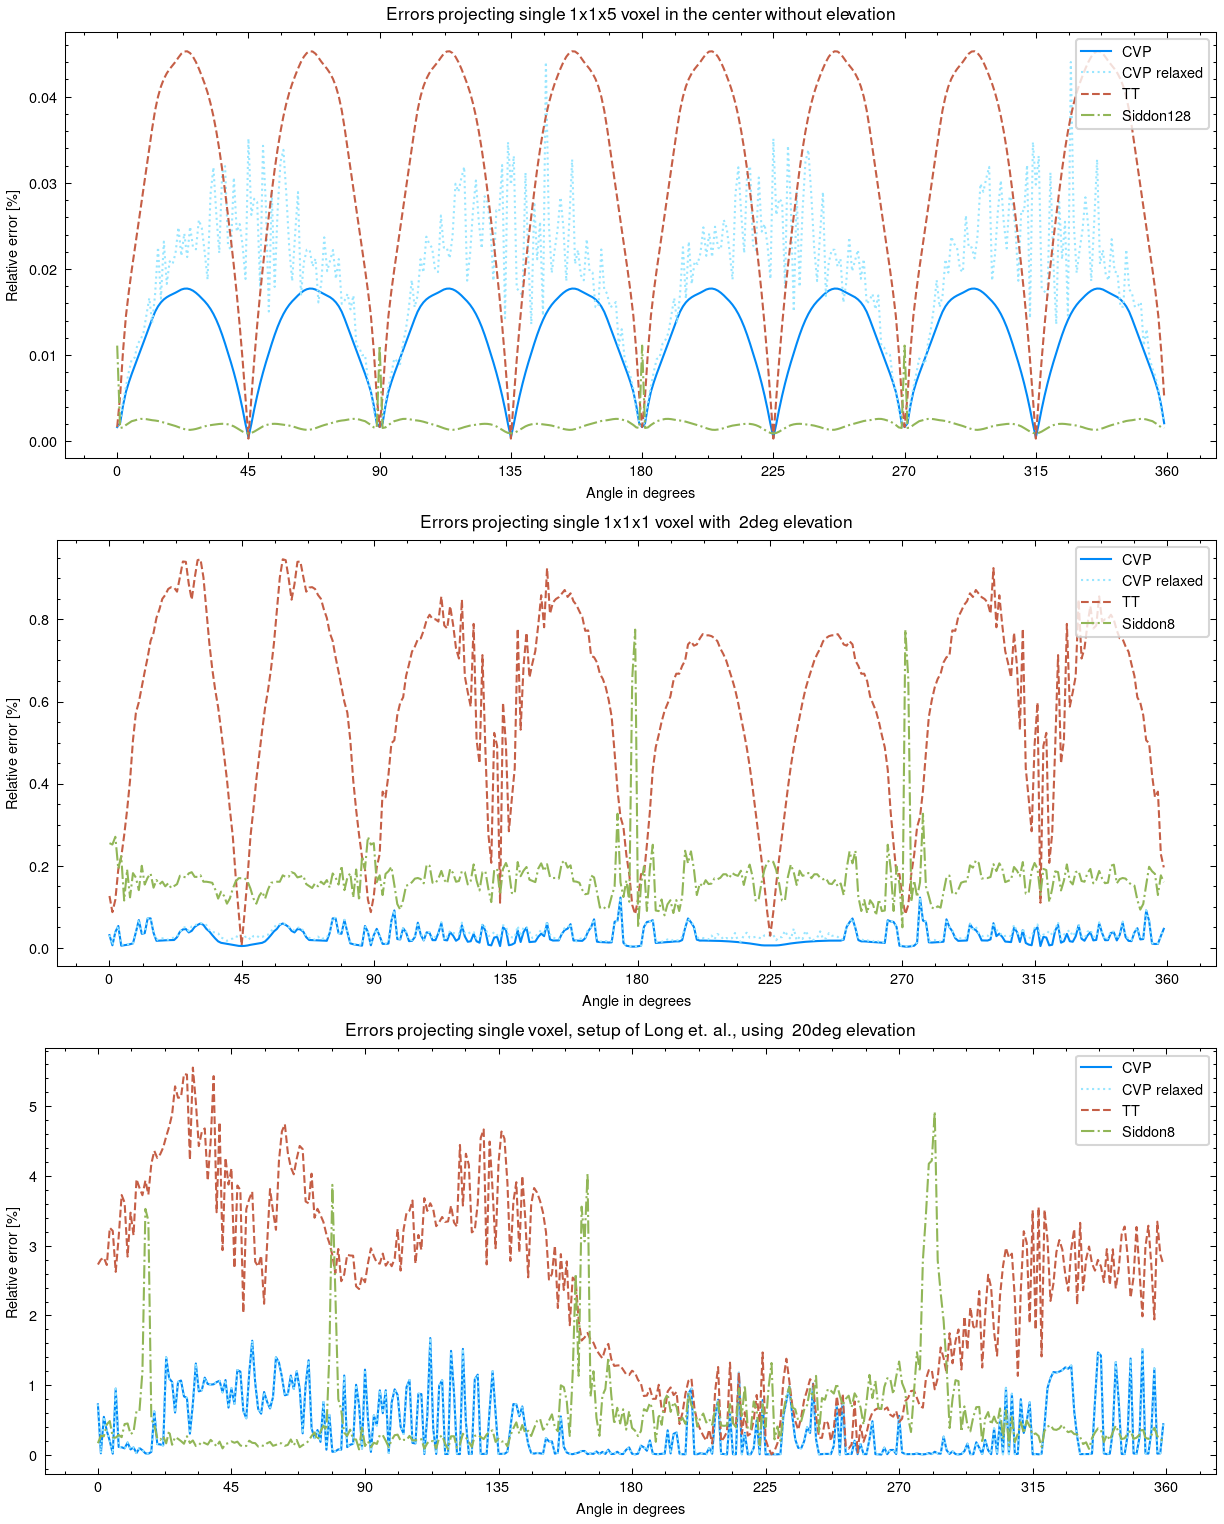
\includegraphics[width=\textwidth]{projectorComparison.png}
    \caption{Comparison of projection errors of different projectors at different settings. In the top image, the voxel is placed in the center of rotation is studied. In the middle image, the voxel is outside rotation center shifted so that the elevation and cone beam angles are around \SI{2}{\degree}. The bottom image shows a setup with  a voxel projected with a large cone beam angles and elevations.}
    \label{fig:projectorerror}
\end{figure*}

% \subsection{Transparency and reproducibility of the results}

% We believe in the concept of open science. Therefore, not only the software developed by the first author is published under an open source license, we are also publishing all the procedures, scripts, input data and log files, including implementation details, that were used to produce the graphs and tables in the results section. This way, anyone can reproduce our steps on their hardware and compare the results, or use our logs and scripts to compare the results with the underlying data. The files and protocols are published on the website \url{https://kulvait.github.io/KCT_doc/categories/cvp-paper-2021.html}.

% This is also important for the users of the software, because in the future we can disclose how the run times of the projectors change with new versions of the software or with new hardware.



%For studying the properties of cutting voxel projector under various scanning settings and discretizations of the volume and  we have chosen two configurations based on the diagnostic trajectories of the Artis Q SIEMENS C-Arm CT system for the brain tomographic scanning, where the distance from the source to the isocenter is $\SI{749}{\milli \meter}$ and the distance from source to the detector is $\SI{1198}{\milli \meter}$. Detector matrix of the device consists of $2464 \times 1920$ detector cells of the dimensions $\SI{0.154}{\milli \meter} \times \SI{0.154}{\milli \meter}$. For the purposes of the tomographic reconstruction there is applied tiling of the pixels, the procedure where the signal is obtained from the merged pixels of the size either $2 \times 2$ or $4 \times 4$.

%Setup I. is derived from the brain scan and uses tiling $2 \times 2$ with merged pixel size of $\SI{0.308}{\milli \meter} \times \SI{0.308}{\milli \meter}$. The trajectory consists of $496$ source and the detector geometrical configurations from which are obtained projection data of the size $1232 \times 960$ pixels. Setup II. is derived from the brain perfusion scan and uses tiling $4 \times 4$ with merged pixel size of $\SI{0.616}{\milli \meter} \times \SI{0.616}{\milli \meter}$. The trajectory consists of $248$ source and the detector geometrical configurations from which are obtained projection data of the size $616 \times 480$ pixels. 

%Siemens was using 0.46433800458908x0.46433800458908x0.46433800458908 voxels in the grid 512x512x325 = 238x238x151
%Siemens was using 0.46433800458908x0.46433800458908x0.46433800458908 voxels in the grid 512x512x394 = 238x238x182
%0.95545232421875x0.95545232421875x0.95545232421875 voxels in the grid 256x256x184 =245x245x175
%(0018, 1100) Reconstruction Diameter = 512 The diameter defines a circular region that is entirely contained within the encoded Pixel Data (7FE0,0010), unless the encoded image has been cropped after reconstruction. 
%As a testing volumes, we have chosen two volumes of the Shepp-Logan 3D like phantom and one volume of the realistic brain phantom, see \cite{Aichert2013}. Shepp-Logan 3D phantom volumes were generated with the voxels that are longer in z-axis direction than xy-axis direction to test this common setup, while the realistic head phantom volume has uniform voxel sizes in every direction so that the volume is in the form proposed by the authors of \cite{Aichert2013}.

%First we have generated Shepp-Logan 3D like phantom of the dimensions $1024 \times 1024 \times 1024$ with the voxel size $\SI{0.215}{\milli\meter} \times \SI{0.215}{\milli \meter} \times \SI{0.215}{\milli \meter}$ that represents the volume of the size $\SI{220.16}{\milli\meter} \times \SI{220.16}{\milli \meter} \times \SI{220.16}{\milli \meter}$. We interpolated this volume to the two different grids of the sizes $256 \times 256 \times 64$ and $512 \times 512 \times 128$ which correspond to the voxel sizes $\SI{0.86}{\milli \meter} \times \SI{0.86}{\milli \meter} \times \SI{3.44}{\milli \meter}$ and $\SI{0.43}{\milli \meter} \times \SI{0.43}{\milli \meter} \times \SI{1.72}{\milli \meter}$ respectively.

%For the realistic brain phantom we have generated the volume by the procedure described in \cite{Aichert2013}. Size of the volume without slices containing zeros is $256\times256\times212$. For voxels of the dimensions $\SI{0.9}{\milli \meter} \times \SI{0.9}{\milli \meter} \times \SI{0.9}{\milli \meter}$ the grid fits into the volume of $\SI{230.4}{\milli\meter} \times \SI{230.4}{\milli \meter} \times \SI{190.8}{\milli \meter}$.


%For each discretized volume and setup we first compute its projections using given projector. Then we run constant number of $40$ iterations of CGLS algorithm for the tomographic reconstruction. Then we study the norm of residuum, norm of error based on the original data and computational time of reference implementation.


%For each volume discretization we first resized original volume and compute projections using given projector backprojector pair.

%We decided to test cutting voxel projector by comparing the reconstructions created using d
